\documentclass[11pt]{article}
\usepackage{etex}
\usepackage[round,longnamesfirst]{natbib}
\usepackage{amsfonts}
\usepackage{mathpazo}
\usepackage{hyperref}
\usepackage{xcolor}
%\hypersetup{
%    colorlinks,
%    linkcolor={blue!75!black},
%    citecolor={blue!75!black},
%}
\usepackage{parskip}

%Idioma
\usepackage[english]{babel}
% define colors
\definecolor{myblue}{RGB}{10, 36, 99}
\definecolor{mywhiteblue}{RGB}{36, 123, 160}
\definecolor{myred}{RGB}{251, 54, 64}
\definecolor{mygrey}{RGB}{96, 95, 94}
\definecolor{mywhitegrey}{RGB}{226, 226, 226}
%\usepackage[colorlinks=true,linkcolor=myblue, allcolors=myblue]{hyperref}
\hypersetup{
	colorlinks,
	linkcolor=myblue,
	citecolor=myred,
	%urlcolor =black,
}

\usepackage{multimedia}
\usepackage{graphicx, color}
%\usepackage{pstricks,pst-node,fancybox,pst-text}
\usepackage{epsfig}
\usepackage{amsthm}
\usepackage{mathtools}
\usepackage{esint}
\usepackage{amssymb}
\usepackage{url}
\usepackage{graphicx}
\usepackage{relsize}
\usepackage{amsfonts}
%\usepackage{fancyheadings}
\usepackage{float}
\usepackage{color}
\usepackage{mathrsfs}
\usepackage{setspace}
%\usepackage{lipsum}
%\usepackage{tikz}
\usepackage[mathscr]{euscript}
\usepackage{caption}
\usepackage{subcaption}
\usepackage{pdflscape}
\usepackage{booktabs}
\usepackage[utf8]{inputenc}
\usepackage[T1]{fontenc}
\usepackage{geometry}
\newtheorem{thm}{Theorem}[section]
\newtheorem{cor}[thm]{Corollary}
\newtheorem{lem}[thm]{Lemma}
\newtheorem{prop}[thm]{Proposition}
\usepackage[bottom]{footmisc}
\usepackage{pgf,tikz}
\usepackage{amsmath,amsthm}
\usepackage{amssymb}
%\usepackage{bbm}
\usepackage{lscape}
\PassOptionsToPackage{normalem}{ulem}
\usepackage{ulem}
%\usepackage{shadethm}

%%Equation%%
%\usepackage{stackrel}
\usepackage{bm}
\usepackage{xr}
%\externaldocument{BHM_AER_online_appendix}

\newenvironment{definition}[1][Definition]{\begin{trivlist}
\item[\hskip \labelsep {\bfseries #1}]}{\end{trivlist}}

\setlength{\topmargin}{-0.4in}
\setlength{\textheight}{8.85in}
\setlength{\oddsidemargin}{-0.2in}
\setlength{\evensidemargin}{0.0in}
\setlength{\textwidth}{6.93in}
\renewcommand{\baselinestretch}{1.44}

\newcommand{\blue}{\textcolor[rgb]{36,60,84} }        % author cite
\newcommand{\skyblue}{\textcolor[rgb]{71,183,196}}    % equation
\newcommand{\blueG}{\textcolor[rgb]{71,132,148}}      % Green
\newcommand{\gray}{\textcolor[rgb]{112,121,120}}      % hh
\newcommand{\brown}{\textcolor[rgb]{108,88,94}}       % eq2

%%%DefineColo%%%%
\definecolor{blue}{RGB}{6,13,51} 					%Author cites
\definecolor{skyblue}{RGB}{71,183,196}		%Equ	
\definecolor{pink}{RGB}{201,90,138}		    %Equ
\definecolor{pant}{RGB}{202,184,154}
\definecolor{BlueG}{RGB}{115,136,174}
\definecolor{skinJ}{RGB}{180,158,161}
\definecolor{purple}{RGB}{122, 37, 190}
\definecolor{gray}{RGB}{111,111,142}

\newtheoremstyle{prop}{18pt}{18pt}{}{}{\sc}{.}{.5em}{}
\theoremstyle{prop}
%\newshadetheorem{prop}{Proposition}

\usepackage{setspace}
\onehalfspacing

\defcitealias{kline2018profits}{KPWZ}
\defcitealias{klineQJE2018}{KPWZ}
\defcitealias{Staiger2010}{SSP}


\renewcommand*\abstractname{Disclaimer}
%~~~~~~~~~~~~~~~~~~~~~~~~~~~~~~~~~~~~~~~~~~~~~~~~~~~~~~~~~~~~~~~~~~~~~~~~~~~~~~~~~~~~~~~~~~~~~~~~~~~~~~~~~~~~~~~~~~~~~~~~~~~~~~~~~~~~~~~~~~~~~~~~~~~~~~~~~~~~~~~~~~
%~~~~~~~~~~~~~~~~~~~~~~~~~~~~~~~~~~~~~~~~~~~~~~~~~~~~~~~~~~~~~~~~~~~~~~~~~~~~~~~~~~~~~~~~~~~~~~~~~~~~~~~~~~~~~~~~~~~~~~~~~~~~~~~~~~~~~~~~~~~~~~~~~~~~~~~~~~~~~~~~~~
% DIRECTORIES FOR ALL FIGURES AND TABLES IN PAPER
\newcommand{\MATLABfigureDir}{../2_MATLAB_code/Created_figure_files/}       % Figures created by MATLAB
\newcommand{\MATLABtableDir}{../2_MATLAB_code/Created_table_files/}         % Tables created by MATLAB
\newcommand{\POWERPOINTplotDir}{./Figures_drawn_in_Powerpoint}              % Figures drawn 'by hand' in Powerpoint and imported as png files (no data or code used)
\newcommand{\EMPIRICALtablesDir}{../3_Empirical_tables}                     % Tables created from Census results / data
%~~~~~~~~~~~~~~~~~~~~~~~~~~~~~~~~~~~~~~~~~~~~~~~~~~~~~~~~~~~~~~~~~~~~~~~~~~~~~~~~~~~~~~~~~~~~~~~~~~~~~~~~~~~~~~~~~~~~~~~~~~~~~~~~~~~~~~~~~~~~~~~~~~~~~~~~~~~~~~~~~~
%~~~~~~~~~~~~~~~~~~~~~~~~~~~~~~~~~~~~~~~~~~~~~~~~~~~~~~~~~~~~~~~~~~~~~~~~~~~~~~~~~~~~~~~~~~~~~~~~~~~~~~~~~~~~~~~~~~~~~~~~~~~~~~~~~~~~~~~~~~~~~~~~~~~~~~~~~~~~~~~~~~

\begin{document} %\sloppy

\title{Summaries on Selected Papers in Migration and Human Capital}
\author{Sany Leon \thanks{
		E-Mail:\ \href{mailto:sany.lcurasi@gmail.com}{sany.lcurasi@gmail.com}}
}
%\date{\today}
\maketitle

%\vspace{-1cm}
%\begin{center}
%	\begin{large}
%\textit{Preliminary and incomplete}
%\end{large}
%\end{center}


\begin{abstract}
\noindent{\normalsize  These summaries review were written to analysis several methods when migration affects human capital and do not necessarily imply the authors' current reading of the literature. I would be happy to correct any errors and misinterpretations as well as entirely remove references to papers.}
\end{abstract}

%\thispagestyle{empty} %\addtocounter{page}{-1}
%\newpage
\addtocounter{page}{-1}

\tableofcontents

\thispagestyle{empty} %\addtocounter{page}{-1}
\newpage

%%%%%%%%%%%%%%%%%%%%%%%%%%%%%%%%%%%%%%%%%%%%%%%%%%%%%%%%
%%%%% SECTION 1
%%%%%%%%%%%%%%%%%%%%%%%%%%%%%%%%%%%%%%%%%%%%%%%%%%%%%%%%

%%%%%%%%%%%%%%%%%%%%%%%%%%%%%%%%%%%%%%%%%%%%%%%%%%%%%%%%
%%%%% SECTION 2
%%%%%%%%%%%%%%%%%%%%%%%%%%%%%%%%%%%%%%%%%%%%%%%%%%%%%%%%
%\vspace*{-.3cm}\paragraph{Literature.}\label{sec:Literature}

%Our work is related to a growing literature that explores the implications of market power.

%%%%%%%%%%%%%%%%%%%%%%%%%%%%%%%%%%%%%%%%%%%%%%%%%%%%%%%%
%%%%% SECTION 4
%%%%%%%%%%%%%%%%%%%%%%%%%%%%%%%%%%%%%%%%%%%%%%%%%%%%%%%%
\section{Theories of Migration}%\label{sec:card1994}

	\subsection{Lee (1966): ``A theory of migration''}
	%Lee, E. S. (1966). A theory of migration. Demography, 3(1), 47-57.
	
	\paragraph{Summary}
	In this paper the author elaborated a migrations schema for to do some hypotheses with to review of the theories of the migration and to attempt the different variables to influenced in the mobility of the people.
	
	Migration is defined as a permanent or semi-permanent change of residence, with spatial mobility from one region to another without considering the distance every act of migration involves an origin, a destination, and obstacles. The continual movement of nomads, migratory workers, and short-term and temporary residents are not considered a migration.
	
	To Analysis the author assumed that exist positive (+) factor \footnote {Positive (+) factor for the place attract to people}, negative (-) \footnote{Negative (-) factor for the place repel people} and neutral (0) \footnote{Neutral (0) factor for none effect} in the original place and the destination.  The factors that affect the migration are: Area of the origin, destination, intervening obstacles and personal factors. In many times not all the people who migrate reach to do. 
	
	\paragraph{Theoretical results}
	The case of children moves with their parent willy-nilly. \textit{The volume of the migration} is related with the public services in some placed and the diversity of the people and this volume increase cause of the diversity concentration. The \textit{stream and counter-stream} of migration , For every major migration stream counter stream develop and the efficiency of the stream is high when exist major factor in development of a migration with minus factor in the origin place and the migration efficiency stream be high if the intervening obstacles are
	great.

	About the \textit{\textit{characteristic of the migrants}}, This said migration is selective, since the migrants are into groups with different reasons and motivations. Responding firstly to the minus factor in the origin place they tend to respond to the plus factor with the destination. If the migrants together put distribution, this tends to be bimodal. The heightened propensity to migrate at certain stages of the life cycle is important in the selection of migrants. Finally, the migrants characteristic is an intermediate-term between the origin and destination place.
	 
	\paragraph{Results}
	As conclusion the author recognizes the important of the intern migration upon the social and economic development of the countries.
	the movement of people may tend to lower the quality of population, as expressed in terms of some particular characteristic, at both origin and destination.
	 
	 \newpage
	 
	\subsection{Ravenstein (1885): ``The Laws of Migration''}
	%Ravenstein E. G., 1885 The Laws of Migration Journal of the Statistical Society of London	48(2), 167–235.
	
	\paragraph{Summary}
	The aim article is to prove the migratory movement with different statistics in different countries with the censuses, notwithstanding its mistake policies. The methodology applied by the author to analyze migration, use the population's parochial, provincial and national element or foreign element like a place who born the people were.
	The information compiled to analyze the article was extended around Europe and North America. 
	
	\paragraph{Theoretical Result} Thus, the place of birth determines this element and people born in some place "x", are considered natives there regardless of their father or mother. The process of migration in the principal countries was represented by the author, e. g. after the huge analysis about migration, it was increasing and just the exception was England caused the interference of the Irish immigrants. Ravenstein used the census information, where the migration increased and the female tend to be the long-journey migrants. 
	
	\paragraph{Conclusion and results} About the stream, the local which carry to rural population toward the cities. 
	Ravenstein consider the temperature (tropical climate and any other), assuming if the origin place climate is similar to the destination so the migrants will thrive and they settled down permanently. 
	
	
	
	\subsection{Card (2005): ``Is the new immigration really so bad?''}
	
	\paragraph{Summary} he author review US immigration literature and planted two question: Do immigrants harm the labor market opportunities of less skilled natives? and how do today’s immigrants perform in the US labor market, and are they successfully being assimilated?.
		
	Firstly the authors describe about \textit{the characteristic of immigrants}, emphasized by {\color{blue} Borjas (1985, 1995)}, the skill characteristics of immigrants in the US are strongly related to their country of origin. For the analysis was measured by the 2000 data census, comparing the educational attainment of natives and immigrants. What stands out in data 200 Census, the immigrant comprised within the working age population was 13\% while this same population with less than a high school was 28\%. Above the education distribution ---at the upper--- between immigrants and natives the author affirmed the immigrants education were slightly more likely than natives to hold an advanced degree. In fact the wage gap between the high school graduate and dropout, had an upward pressure exerted by the immigrants inflow and downward pressure on the college–high school wage gap.
	
	\paragraph{Analysis and models}
	%The conclusion when the labor market competition from immigrants is most intense for natives with the lowest levels.
	
	The \textit{immigrant competition and the labor market outcomes of know skilled natives}, was studied since the impact of the immigration on native workers with {\color{blue} Grossman (1982)}. Consequently it appropriated establishing the relate differences in the relative structure of wages in different local labor markets to differences in the relative supply of immigrants and on the other side is a time series method, relating changes over time in immigrant densities to economy-wide measures of relative labor market outcomes.
	
	According {\color{blue}(Jaeger, 1996; Card, 2001)}; the adequate manner to evaluated the impact of immigration is assuming that within skill group ---immigrants and native--- also are perfect substitutes, where firstly evaluate the effect of immigrants on the relative supplies of different skill groups in different cities, and the next step is relate the relative wages for different skill groups to the relative supplies in the local labor market.
	
	Therefor the \textit{effects of immigration on relative supply of low skilled labor}. Since comparing the fraction of dropouts in the adult population and the fraction of immigrant dropout in local adult population, the share of dropouts in the local working-age population in the city $c$, {\color{skyblue}$\bm{s^d (c)$}} is is the sum of the share of native dropouts $s^dN(c)$ and the share of immigrant dropouts, $s^dl(c)$, with $e(c)$ is a residual
	\begin{equation}
		{\color{skyblue}\bm{s^d (c)}} = \alpha + \beta s^dl(c) + e(c)
	\end{equation}
		%%The intuition%%
	If the less educated immigrant inflow is offset by the native dropout outflow, this will result in: The immigration impact will be slightly on the overall dropout share and
	the coefficient $\beta$ will be close to 0 and for $\beta$ equal to 1, There are uncorrelated between the mobility flows of native dropouts and the inflow rate of low skilled immigrants. The model is more consistent with a value of $\beta$=1 than $\beta$= 0 ---the slope is set to 1---.
		%%Result%%
	The author concluded, about the relative supply impact of immigrant studies had an output with a bigger effect on local labor markets.
	
	To continue the analysis the\textit{ impacts on less skilled natives}, was measured by the author with the local production function and set of per capita labor supply of each skill group, implicating the relative wages and relative employment rates of workers, e.g. when comparing the high school graduates to dropouts, a relative supply-demand the model being:
	
	\begin{subequations}
		\begin{equation}
			log (\hm{w^d/w^H}) = a_1 + b_1log(s^d/s^H) +u_1 
		\end{equation}
		\begin{equation}
			log (\hm{E^d/E^H}) = a_2 + b_2log(s^d/s^H) +u_2 
		\end{equation}
	\end{subequations}
	where $w_d$ and $w_H$ are the mean wages of dropouts and high school graduates in a city, $E_d$ and $E_H$ are the mean employment-population rates of the two groups, and $s^d$ and $s^H$ are the shares of dropouts and high school graduates in the local population. The coefficients $b_1$ and $b_2$ depend on the elasticity of substitution between skill groups $(\sigma)$ and on the elasticity of the per-capita labor supply functions $(\epsilon)$:
	
	\begin{subequations}
		\begin{equation}
			b_1=-1/(\sigma+\epsilon), b_2 = -\epsilon / (\sigma+\epsilon) 
		\end{equation}
	\end{subequations}
	
	With the$(\epsilon=0)$ the local labor supplies are perfectly inelastic then occur that $log (w^d/w^H)$ reduces to the familiar model used in studies of education-based wage gaps {\color{blue}(Katz and Murphy, 1992)}.
		%%Intuition%%
	Respect to two equation $log (w^d/w^H)$ and $log(E^d/E^H)$ , the {\color{blue} Hecksher-Olin} style model for the local economies approach the relative wage and the relative labor supplies are may be uncorrelated.
		%%Result%%
	For the local demand-supply system te formal output estimated by OLS, there is not exist between high school dropout relative wage and their relative supply. 
	
	\paragraph{Conclusion}
	%%General Conclution%%
	Finally, the author does a remarkable conclusion, showing evidence that the children (who were born in US) of the immigrants parents are higher education, especially in the second and third generation, and considering the human capital parents, those children did well. 
	
	The low-skilled native was not affected by the relative supply shock immigrant, although strong effect immigrant on the relative supply. "The relatively strong educational progress of second-generation immigrants, together with the limited evidence of adverse effects on less-skilled natives, suggest that the new immigration may not be so bad after all". Also, the evidence shows, that unskilled immigrants have a place in countries with industries with high immigrant rates.
		
	
\section{International Migration}
	
	\subsection{Yap (1976): ``Internal migration and economic development in Brazil''}
	%Yap, L. (1976). Internal migration and economic development in Brazil. The Quarterly Journal of Economics, 90(1), 119-137
	
	\paragraph{Summary}The study’s aim is the relationship generated in the internal migration —social impact— and the economic growth in Brazil, in this case the rapid urban population growth; in general, the focus is rural-urban migration. The author wondered above the effect the huge migration —rural to urban— after the World War II with the general equilibrium framework. The Brazil’s economic growth, where the income has risen —having a positive effect on the wage distribution. The migration rural-to-urban migration shown has had social gain, however there is rural and urban poverty. Despite the fact their relatively more earn than the in the rural area, their absolute income are low and they access to the social services limited.
	
	\paragraph{Model} This used a three-sector model to measure the Brazilian migration, implying the model of Lewis, and Fei and Ranis with simulation techniques to quantify the impact of migration. Migration is a endogenous variable. The model begins with the 1950 population census and national account ending in 1965.
	
	\paragraph{Results} The model applied shown that the migration has a positive relationship after the Brazil’s postwar development. To the extreme when the migration is prohibited —mind the population growth rates remain almost constant — the average growth Brazil reduces. The logit model used the conditional fixed effect on school attendance and primary school completion. His finding of child migration has had a positive impact on child school attendance rates, however; completion of primary school was not affected by school attendance.
	
	%%%%%A PAPAER FOR UGANDA CASE%%%%%%%
	%%%%The migration study in Uganda cause of the intense flows of internal mobility also the international migration boosted by the demographic, economic and political factors and the armed conflict, using the Uganda’s Panel Survey data for 2005, 2009, 2010 and 2011 (basically finding that in 2000s the 20 per cent household have at least one member with migration experience).
	 
	\subsection{Dustmann (2007): ``Return Migration: Theory and Empirical Evidence from the UK''}
	%Dustmann, C., \& Weiss, Y. (2007). Return Migration: Theory and Empirical Evidence from the UK. British Journal of Industrial Relations, 45(2), 236–256.
	The paper objective is demonstrating the migration is temporary rather than permanent, based on this the main question is, why the immigrants should return? The migration takes different forms, the two main reason is economic motives —implies temporary and permanent migration and natural disaster or persecution—. Permanent migration occurs if at the end of the migrant’s lifetime, benefits are still higher than costs.
	The model considers two decisions around the migrant: whether or not to emigrate and whether or not to return to the home continuing working for to measure their productive, and neglect cost of migration and uncertainty about future wages and assume a world of perfect foresight.
	Using data from UK. It shown that the return migration is explicated by subjective variable —preferences for consumption in their country— or high purchasing power host country’s currency respect the migrant’s home country, or knowledge acquire migrants had as result the rising their productivity in their country home. All this introduce heterogeneity in the immigrant behavior. 
	
	\subsection{Smith (2015, \textit{Handbook of the Economics of International Migration, Chapter 4}): ``The Human Capital (Schooling) of Immigrants in America''}
	%James P. Smith, Chapter 4 - The Human Capital (Schooling) of Immigrants in America, Editor(s): Barry R. Chiswick, Paul W. Miller, Handbook of the Economics of International Migration, North-Holland, Volume 1, 2015, Pages 183-210
	The authors pretend to explain the human capital (schooling) of immigrants from United State. The human capital is represented by the schooling years of the migrants using also the heterogeneity migrants and they wondered above the disparity education on the nativity. 
	The methodology used the Current Population Survey (CPS) from the 2002 and 2010, contrasting three groups, the foreign born, native born and recent foreign born. The USA immigration have less schooling than the native born the female migrants trail male migrants by about one-tenth of year of schooling. 
	
	On the other hand, the Latino migrants are much less competence than the native-born including less European or Asian migrant —it could be explicated by the years schooling, since just the 30\% have only eight years of schooling. The diversity (this implies the heterogeneity) is another variable that influenced on the migration. The authors highlight the importance of the education on the policy public— also to controlled the correct manners of the legal migration—. The European and Asian new migrant have more schooling than the native born.
	
	\subsection{Korpi (2015): ``Internal migration and human capital theory: To what extent is it selective?''}
	%Korpi, M., \& Clark, W. A. V. (2015). Internal migration and human capital theory: To what extent is it selective? Economics Letters, 136, 31–34
	La investigación sobre la migración laboral interna, sugieren que los migrantes se desplazan para mejorar los rendimientos de su trabajo, a partir de deducción de las principales encuestas internacionales mostraron que menos de un tercio de los migrantes internos están motivados por fuerzas laborales. 
	
	Los autores se cuestionan sobre el rendimiento de la migración, ¿las ganancias en ingresos uniformes a lo largo de la distribución del ingreso? y ¿cómo este resultado depende de los antecedentes educativos de los inmigrantes y de la dirección de su migración?.
	
	La metodología por MCO aplica variables de interés como: nivel de educación alcanzado de acuerdo a lugar --–metropolitano o regional–-- edad, ingreso y empleo; con datos de panel sobre hogares unipersonales. Los resultados del emparejamiento CEM inicial y la regresión por cuartiles sugieren que los grandes retornos de la migración interna son captados principalmente por las personas con mayor educación, las que inicialmente tienen una distribución de ingresos baja y las que se dirigen a las regiones metropolitanas más grandes.
	
	La mayoría de los migrantes internos con grados de educación superior, poseen mejor ingreso que los no migrantes independientemente del lugar de destino y ello se explica por el grado de desempeño del migrante que por supuesto es mejor, no obstante; las ganancias para los migrantes son limitados y en algunos casos tiende a ser negativas. El dinero y los ingresos muestran un margen marginal decreciente típico, esto quiere los beneficios de la migración disminuyen (a medida que se avanza en la distribución de ingresos), si se habla de personas acomodadas. Gran parte de los resultados de la migración son a menudo negativos en términos de rentabilidad. Esto sugiere que los modelos de resultados promedio son insuficientes para abordar la migración motivada por el capital humano.
	
	\section{Internal Migration}
	
	\subsection{Aydemir \& Torun (2022): ``The effect of education on internal migration of young men and women: incidence, timing, and type of migration''}
	%Aydemir, A. B., Kırdar, M. G., \& Torun, H. (2022). The effect of education on internal migration of young men and women: incidence, timing, and type of migration. Labour Economics, 74, 102098.
	
	\paragraph{Summary}
	The compulsory schooling reform in Turkia to demonstrating the causal effect of education on the incidence and internal migration (like a timing exactly). It was analysis with two datasets (2009 to 2017 cross-section), of the turkish household labor force survey and turkish demographic and health survey, these provided information above the education attainment, migrations and labor market. Firstly, a strong political effect on the high school competition (for men and women) is found –this spillover effect is fundamental to explain the effect of education on the migration– because of while the education rises the migration this tend to decline for other reasons. 
	
	\paragraph{Result} The outcome indicated the women acquire high education, if they decide to move another place (within provinces). In fact the evidence shows the education generate an effect sustainable on the ever-migration –--around mind-20’s for men but not for women–-- nerveless the education don’t change the migration incidence on mid-20 s for men and the women prefer to migrate at earlier ages. 
	
	\subsection{Dong \& Zhang (2021): ``The cumulative impact of parental migration on schooling of left-behind children in rural China''}
	%Dong, Y., Wang, W., Li, S., \& Zhang, L. (2021). The cumulative impact of parental migration on schooling of left-behind children in rural China. Journal of Rural Studies, 86, 527-541.
	In this research, the authors pretended to show the impact of parental migration (for off-farm employment) on the schooling years of left behind (during the elementary and junior high school). The data used was of the China Rural Development Survey for the 2005, 2008, 2012 and 2016, considering the characteristic of family. The methodology is divided both the OLS –with the family fixed effect– and Feed Forward equalization, 	
	The parental migration rises the children’s educational investment but it not has effect on the schooling years left-behind children y using the OLS and FFE estimation methods, this study concludes that the accumulated years of parents’ migration for off-farm employment during the child’s elementary or junior high school education stages have no negative effect on the children’s schooling years. By using the FFE estimation method, we have also tried to address endogeneity issues to some extent.
	The effect of parents’ migration experiences on their child’s decision to attend high school: Results from LPM-FFE estimation. %Child has achieved education of high school or above (1 = yes). 
	The accumulated years of mother’s migration during child’s elementary school education stage.
	
	\subsection{Ding (2021): ``College education and internal migration in China''}
	%Xiaozhou Ding, College education and internal migration in China, China Economic Review, Volume 69, 2021
	In this paper the objective is examine the impact of the education of college education on the migration, out of the province into China. They used the data from the China Family Panel 2010 –is a longitudinal survey of ISSS Pekin– and collected data from China Yearly Statistical Book for the number of institutions. The methodology recognizes the variables, urban population, GDP per capita, and the total number of non-farm employment. The key variables have relationship residence province –proxy, cause is the province different from the province when he or she lives at twelve years old–, the author convert the variable to do homogeneous to calculated the model.
	
	The empirical evidence shows that positive relationship among university education and the long-distance mobility into China. Is to say the college education has heterogeneous impact over the migration depending the gender, occupation and childhood’s people.
	
	
	\subsection{Higa, Nonaka, Tsurumi \& Managi (2019): ``Migration and human capital: Evidence from Japan''}
	\paragraph{Summary}
	The authors applied a modified gravity model for Japan municipal-level to examine the domestic migration drivers with the age group of analysis were 0–9, 10–19, 20–29, 30–39, 40–49, 50–59, and 60 or above, with 3,491,292 observation and 1869 municipalities, some of these municipalities don not have migration. The dependent variables was the internal migration several data and the independents variables were: core gravity
	terms in the gravity model, human capital stock and human capital-related variables, variables reflecting the economic conditions of municipalities, variables related to access to public services, indicators of quality, and dummy variables linked to municipal government.
	
	The paper's objective on the effect of the municipalities' human capital stock, to measured as a share of university graduates in te municipal population, and the human capital-related variables, measured as the shortage of nursery school capacity and educational support by a municipal government.
	
	\paragraph {Model} The gravity model serve to analysis the  municipal-level migration, that is:
	
	\begin{equation}
		{\color{BlueG}\hm{M_{ij}}}=Gx\frac{P_i^\alpha x P_j^\beta }{D_{ij}^\gamma}
	\end{equation}
	$M_{ij}$ the population inflow from municipality $j$ to municipality $i$, indicating the $P$ population, and $D$ distance between municipalities, taking the parameters $\alpha \beta \gamma$ with $G$ constant. To study the effects of migration determinants, focusing on the effect of the human capital and the human capital-related variables, applying the estimation model of Andrienko and Guriev.
	\begin{equation}
	\begin{split}	
		ln {\color{BlueG}\hm{M_{ij}}} &= \beta_0 + \beta_1lnP_j +\beta_2 \Delta lnP_{ij} +\beta_3 ln \Delta D_{ij} \\		
				&+\beta_4 Neighboring \thinspace Municipality_{ij} + \beta_5 Within\thinspace Prefecture_{ij} \\
	    		&+\beta_6 \Delta Share\thinspace of \thinspace University Graduates_{ij} +\beta_7 \Delta Shortage\thinspace Rate\thinspace of \thinspace Nursery \thinspace School \thinspace Capacity_{ij} \\
				&+\sum_{n=1}^{N} \gamma_n (X_{in}-X_{jn}) + \sum_{m=1}^{M} \delta_m X_{im} + u_{ij}  
	\end{split}		
	\end{equation}
	where, $ \Delta lnP_{ij}$ is the difference in the populations of the two municipalities, $Neighboring\thinspace Municipality_{ij}$ is a dummy variable indicating that $i$ and $j$ are neighboring municipalities, as well as the variable $Within\thinspace Prefecture_{ij}$ is a dummy to indicate that $i$ and $j$ are located in the same prefecture.
	The Term $X_n$ includes a set of municipal demographic characteristics related to economic conditions, and $X_m$ includes dummy variables such as government support in
	municipality $i$ and dummy variables for the prefecture to which municipality $i$ belongs.
	
	\paragraph {Result} The authors shown that the people tend to migrate from lower human capital stock municipalities to high human capital stock, they are a positive relationship between the universities graduates and the population inflow to municipalities that contain high share of university people ---with a proportion of 1\% to 0.06\% respectively---. In case with zero migration, the population inflow receive just a tiny change cause of the increase of 1\%  in the share of university graduates. The opposite effect is to say when the migration happens is the inflow people increase to 51.
	
	Secondly, for 20–39 age groups analyzed the impact of the differences in human capital is larger, means that they are likely to be active in the labor force. The partners with children prefer to live in a municipality with the better school systems. The final outcome, indicate the policy adequate specifically in education could mitigate the depopulation of urban region where tend to migrate, so the unequal aging smoothed. 
			
	\subsection{Dustmann \& Glitz (2011, \textit{Handbook of the Economics of Education, Chapter 4}): ``Migration and Education''}
	%Christian Dustmann, Albrecht Glitz,	Chapter 4-Migration and Education, Editor(s): Eric A. Hanushek, Stephen Machin, Ludger Woessmann, Handbook of the Economics of Education, Elsevier, Volume 4, 2011, Pages 327-439.
	\paragraph{Summary}
	In this section of the handbook, its important determinate the migration's factor. On the first affirmation, the human capital is formed after the migration and depend of the host and original country. In many time the migrant take the decision to return to the home country, but not before to investment in the human capital ---acquiring new skills---, in other words the outcome of the return is the human capital.
	Its generated the simple model of return migration and investment in human capital. The model want to show the decision process to take the decision to emigrate and how its linked the human capital --the understanding of the human capital come of the earning analysis reflecting the human capital investment.
	
 	\paragraph {Model and intuition} 
 	
 	The model proposed, comprise three times {\color{BlueG}period 1} individuals live in home country, the {\color{BlueG}period 2} individuals live either in the home or in the host country and the {\color{BlueG}period 3} has length $\bm{T}$, defined as the rest of time life until the individual death. and assuming the lifetime is finite with the life duration {\color{orange}$\hm{T+2}$}. while the other two periods dedicate to learning time, the first period is dedicate how acquire education, ---considering the cost--- while do not work in the original country, the second time could be tie to emigrate or not and can decide to acquire more time to education.

	Above \textit{Skill Enhancement and Return Decisions of Migrants}, to maximizes the earning in the  {\color{BlueG}period 2} and {\color{BlueG}period 3}, through choosing the optimal investment in {\color{BlueG}period 2}, $\bm{s^*_D}$ with the optimal time to return $t^*$: 
	\begin{equation}			
	\underset{s,t}{max}^D= {\color{purple}{\omega_D}} X(1-s)+t[{\color{purple}{\omega_D}} (X+ {\color{gray} f(s,A,X)} )] + (T-t)[ {\color{pink}{\omega_O}} (X+\gamma (t) {\color{gray} f(s,A,X)})]  
	\tag{1}
	\end{equation} 

 	with $\omega_j= {\color{pink}O},{\color{purple}D}$ like a rate to return of human capital $X$ acquired in the {\color{BlueG}period 1} at home country ${\color{pink}O}$,  in either origin country ($\omega_j$) or destination country ${\color{purple}D}$. The function ${\color{gray} f(s,A,X)}$ that translates human capital investment $s$ in the host country in the {\color{BlueG} period 2} into skills and $A$ is taken as the ability of the individual.
 	The parameter ${\color{pink} \omega_O}\gamma(t)$ is the rate of return to human capital acquired in the host country back in the home country.
 	
	When the individual decide not to migrate ---within {\color{BlueG}period 2} and {\color{BlueG}period 3}---, thus decides investment in the human capital on second period, $\hm{s^{*}_O}$:
	\begin{equation}
	{\color{pink} \underset{s}{maxF}^O}=\omega_OX(1-s) + T [\omega_O(X+g(s,A,X))]         \tag{2}
	\end{equation}
	$g(s,A,X)$ translates human capital investment in the home country in the second period into skills and is subject to the same standard assumptions as ${\color{gray} f(s,A,X)}$.
	
	The \textit{Skill Investment in the Home Country}, after having chosen the optimal duration abroad $t*$ with and the optimal investment in learning $s*$ where we denote the payoff of these choices as $F^D(t^*,s^*_D)$ in case of emigrating and $F^O(s^*_O)$ In case of not emigrating. X, the human capital stock after the first period,is a function of first-period investment $i:X =X(i)$.
	
	\begin{equation}
		V^D={\color{purple} \underset{i}{maxF}^D}(s^{*}_D, t^*(i), i)- {\color{skyblue} C(i,A)}      \tag{3}
	\end{equation}	
	
	where the education investing in home country is: ${\color{skyblue} C(i,A)}$, the equation when the individual remain in the home country.
	\begin{equation}
		V^O={\color{pink} \underset{i}{maxF}^O}(s^{*}_O(i), i)- {\color{skyblue} C(i,A)}           \tag{4}
	\end{equation}	

		
	\textit{The migration decision}, will depend on the optimal value function:
	\begin{equation} 
	 V=max[V^D-k+ \eta_D, V^O +\eta_O]      \label{5}
	\end{equation}	
	where $\eta_j=O,D$ is the iid extreme value distributed error capturing heterogeneity in the chose, $k$ value of the cost of migration, so the probability to migrate is: $\bm{Prob_{migrate}} = \frac{1}{1+e^(V^O+k-V^D)}$ . For G distribution with the support $[O, \overline{A}]$, the people who migrate from O country to D country is given by: 
	
	$\bm{Proportion_{migrate}}=\int \limits_{x=0}^{\overline{A}}Prob_{migrate}(A)dG(A) $
	for the permanent migration $t=T$, thus this assume $\gamma=1$,  $\gamma'=0$ and $\omega_D>\omega_O$: is the human capital acquired abroad has the same value at home, is to say the the value of human capital is the same (constant) and the capital human rent is higher in the host country.

	\textit{The optimal investment in Human Capital and the optimal migration duration}, consider the problem of the individual at the beginning of the second period. For those who do not migrate, the optimal investment in the second period $s^*_O$:	
	\begin{subequations}
	\begin{equation}
		\frac{dF^D(s,t)}{ds}: -\omega_DX + F_s[T\omega_D +(T-t) \gamma(t) \omega_O] = 0 
	\end{equation}
	\begin{equation}
		\frac{dF^D(s,t)}{ds}: -\omega_D(X + f(.)) - \omega_O (X+ \gamma(t)f(.)) +\omega_O(T-t)\gamma'(t)f(.)= 0
	\end{equation}
	\end{subequations}
	%intution
	The permanent migration occur when $t=T$, assuming $\gamma=1$, $\gamma'=0$ mean the human capital acquired abroad have the same value at the hometown with the human capital rate higher $w_D >w_O$. The optimal investment in human capital during the {\color{BlueG} period $2$} is $\omega_OX = \omega_Df(s)T$ mean without consider the earning in {\color{BlueG} period $2$}, the profits lost in the second period are equal to the profits from the investment in human capital in the {\color{BlueG} period $3$}. 
	
	Taking the function $f(.)$ , the human capital investment $\hm{s}$ increase in $T$ and investment may change when the human capital stock X upon arrival. The wage change between {\color{BlueG} period 2} and {\color{BlueG}3} is given by $\Delta w_D= \omega_D(f(.) + \hm{s}X)$, this mean with investment $\hm{s}$, wages grow faster the higher the skills the individual has upon arrival

%%subtittle%%
	The \textit{Temporary Migration with Exogenous Return Date}, denoting $\overline{t}$ like exogenous set migration duration the optimal investment in skills $\hm{s}$ is chosen so $\gamma(\overline{t})= \gamma< \frac{\omega_{D}}{\omega_{O}}$, thus the human capital acquired in the host country is less valuable when the individual back home.
	\begin{equation}
	-\omega_{D}X + f_s [\overline{t}\omega_{D}+(T-\overline{t}) \gamma \omega_{O})] = 0   \tag{7b}  
	\end{equation} 
%%subtittle%%
	For \textit{the temporary migration with Endogenous Return Date}. Begin of the choice of optimal second-period investment $\hm{s}$ with endogenous return, the optimal migration period is since by:
	\begin{equation}
	\omega_D(X + f(.)) - \omega_O (X+ \gamma(t)f(.)) +\omega_O(T-t)\gamma'(t)f(.)= 0
	\end{equation}


	%The movement immediate and postponed migration could be represented by the graph 
	
	
	%%%%%%%%Grafico%%
		\tikzset{every picture/.style={line width=0.75pt}} %set default line width to 0.75pt        
		
		\begin{tikzpicture}[x=0.75pt,y=0.75pt,yscale=-1,xscale=1]
			%uncomment if require: \path (0,310); %set diagram left start at 0, and has height of 310
			
			%Shape: Axis 2D [id:dp6752786097780794] 
			\draw  (27.26,150) -- (241.65,150)(27.26,17) -- (27.26,150) -- cycle (234.65,145) -- (241.65,150) -- (234.65,155) (22.26,24) -- (27.26,17) -- (32.26,24)  ;
			%Straight Lines [id:da6193345319531156] 
			\draw    (28.2,116.99) -- (57.86,116.99) -- (237.14,116.99) ;
			%Shape: Parabola [id:dp4697321998319077] 
			\draw   (232.19,58.16) .. controls (144.15,56.51) and (75.97,69.17) .. (27.64,96.14) ;
			%Shape: Axis 2D [id:dp14640900665761558] 
			\draw  (382.75,152.66) -- (597.14,152.66)(382.75,19.66) -- (382.75,152.66) -- cycle (590.14,147.66) -- (597.14,152.66) -- (590.14,157.66) (377.75,26.66) -- (382.75,19.66) -- (387.75,26.66)  ;
			%Straight Lines [id:da9036343965852534] 
			\draw    (382.69,114.65) -- (412.36,114.65) -- (591.63,114.65) ;
			%Shape: Parabola [id:dp096124870099348] 
			\draw   (587.68,97.81) .. controls (499.64,96.16) and (431.45,108.82) .. (383.13,135.8) ;
			%Straight Lines [id:da12456558652922123] 
			\draw  [dash pattern={on 0.84pt off 2.51pt}]  (435.17,114.43) -- (435.17,152.43) ;
						
			% Text Node
			\draw (429,153) node [anchor=north west][inner sep=0.75pt]  [font=\scriptsize] [align=left] {t*};
			% Text Node
			\draw (370,153.01) node [anchor=north west][inner sep=0.75pt]  [font=\scriptsize] [align=left] {t*=0};
			% Text Node
			\draw (586.14,157.38) node [anchor=north west][inner sep=0.75pt]  [font=\scriptsize] [align=left] {t};
			% Text Node
			\draw (452.65,121.4) node [anchor=north west][inner sep=0.75pt]  [font=\tiny]  {$Marginal\ gain:\ \omega _{D}( X+f( .))$};
			% Text Node
			\draw (406.17,62) node [anchor=north west][inner sep=0.75pt]  [font=\tiny]  {$ \begin{array}{l}
					Marginal\ Cost:\\
					\omega _{O}( X+\gamma ( t) f( .) -\omega _{O}( T-t) \gamma '( t) f( .))
				\end{array}$};
			% Text Node
			\draw (14.51,152.36) node [anchor=north west][inner sep=0.75pt]  [font=\scriptsize] [align=left] {t*=0};
			% Text Node
			\draw (229.65,156.72) node [anchor=north west][inner sep=0.75pt]  [font=\scriptsize] [align=left] {t};
			% Text Node
			\draw (118.16,118.74) node [anchor=north west][inner sep=0.75pt]  [font=\tiny]  {$Marginal\ gain:\ \omega _{D}( X+f( .))$};
			% Text Node
			\draw (62.68,29.34) node [anchor=north west][inner sep=0.75pt]  [font=\tiny]  {$ \begin{array}{l}
					Marginal\ Cost:\\
					\omega _{O}( X+\gamma ( t) f( .) -\omega _{O}( T-t) \gamma '( t) f( .))
				\end{array}$};
			
			\end{tikzpicture}
		
	Now the individual choose, \textit{the optimal investment in learning in the first period}, first is assumed the individual begin with a base level of productivity, where the including the compulsory schooling: $X(0)=X^0$, so the optimal investment when the individual migrant:
	\begin{subequations}	
	\begin{equation}
	{\color{purple}{\omega_D}}(1-s^{*}_D(i))X_i + t^*(i){\color{purple}{\omega_D}}(1 + f_X)+(T-t^*(i)){\color{pink}{\omega_O}}X_i(1 + \gamma (t^*(i))f_X) = B^D(i)={\color{skyblue} C(i,A)}
	\end{equation}
	and when do not exist the migration this is:
	\begin{equation}
		{\color{pink}{\omega_O}}(1-s^{*}_O(i))X_i + T{\color{pink}{\omega_O}} X_i(1+gx)=  B^O(i)={\color{skyblue} C(i,A)}
	\end{equation}
	\end{subequations}
	where $X_i =\frac{\partial X}{\partial i}$. Thus, in the migration case, the individual will compare the marginal cost of investing in the first period. if the migration decision of the individual is based on a comparison of $V_D-k$ and $V_O$.  In his model, individuals have an (exogenous) probability of migrating $\phi$ so that the optimal investment is given by:
	
	\begin{center}
			$( \pi \omega_{D} +(1-\phi)\omega_{O}) X_i(1-T) ={\color{skyblue} C(i,A)} $
	\end{center}

	For optimally chosen $s^*$ and $t^*$ the value of migrating is sufficiently higher than the value of nonmigrating, then individuals will invest in education in the home country to obtain the critical level of $X^{min}$ that then allows an emigration in the next period, given that
 	\begin{center}
 	$V_D-k |_{X(i)\geq X^{min}} > V^O$
 	\end{center}
	For instance,
	PhD studies in the United States may require a Bachelor’s degree in the country of origin. In that case, optimal investment in the home country will take this requirement into account.
		
	\subsection{Borjas (2015, \textit{Book of Immigration Economics, Chapter 8} ): ``High- Skill Immigration''}
	%
	Borjas recall  abording the caconical model of a competitive labor market, where the receiving country of immigrants, receives a superficially scarce net economic benefit, including if we consider the influx of high-skill worker, not increase the gains. notwithstanding the exposouring of native individual with hight-skill immigration, triggering to increasing the human capital, this mean the human capital generate externality.
	
	\textit{Model of Immigration and Human Capital Externalities}
	Taking the production function, where its depend the stock ideas 
	$A$ is the stock ideas, $K$ is the capital stock and $L$ represents the high-skill workers. The constant return are $K$ and $L$ and $\phi$ gives the externalities elasticity associated with a 1 percent increase on $A$.
	\begin{equation}
		Y= A^\phi[K^\alpha L^{1-\alpha}] 		
	\end{equation}
	
	\noindent Naturally the ideas $A$ and workers $L$ change proportionally (so $A$=$L$). Thus the high- skill immigrant marginal product is:
	\begin{equation}
		MP_L= (1+ \phi -\alpha)K^\alpha L^{\phi-\alpha}		
	\end{equation}
	Mean the influx immigrants increase both the ideas the numbers of workers. 
	
	The high-skill worker marginal product change is:
	\begin{equation}
		dlog MP_L= \begin{cases}
			(\phi-s_k)m,
			& if\thinspace d\text{log}K=0\\
			\phi m, 	& if\thinspace d\text{log}K=m.
		\end{cases}
	\end{equation}
	$m = d$log$L$; and $s_K$ is the capital’s share of income.
	Representing the spillover effect and the law of diminishing returns in the short run and if $\phi$ is huge the value of marginal product of high- skill workers rises. the marginal product of high-skill workers must rise in the long run aft er the capital stock fully adjusts to the high- skill supply shock.
	
	\textit{The Labor Market for Doctorates}
	After empirical evidence, the doctoral degree have an positive effect on the foreign student who get impact on the high-skill worker supply. The persons (foreign-born) granted in the year $c$ and the discipline $d$, Shown by: $p_{sd}= \frac{M_{cd}}{M_{cd} + N_{cd}}$. With $M_{cd}$ like a immigrants and $N_{cd}$ natives. 
	
	The effect of the immigration on the native-born doctorates earning, is: 
	\begin{equation}
		\text{log} w_{cd} (t)=\phi_c+\phi_d+\phi_t+\phi_{ct}+\phi_{dt}+\phi_{cd}+ \theta p_{cd} + \epsilon 		
	\end{equation}
	
	$w_{cd} (t)$ is the mean annual earnings at time $t$  of workers who 
	obtained their doctorate in calendar year $c$ and $d$ discipline  while $\phi_c, \phi_d, \phi_t$, and $\phi_{ct}$ are vectors to measure the fixed effect.
	$\phi_{ct}$ and $\phi_{dt}$ are the possibility to wages change a long the time for the "particular cohort". the $p_{cd}$ is the immigrant share for each of these cohort- discipline with the coefficient $\theta$.
	
	\subsection{Adrienko \& Guriev (2004): ``Determinant of interregional mobility in Russia''}
	
	

	\subsection{Greenwood (1997, \textit{Handbook of Population and Family Economics, chapter 12}): ``Internal migration in developed countries''}
	
	\textit{Gravity and modified-gravity model} The gravity model was modified first giving the behavioral content to the model and additional influences variables' within the estimated relationship. 
	
	\begin{equation}
			\begin{split}	
			ln {\color{BlueG}\hm{M_{ij}}} &= ln\beta_0 + \beta_1lnD_{ij} +\beta_2 lnP_i +\beta_3 ln P_j \\		
			& +\beta_4 lnY_i + \beta_5 lnY_j +\sum_{n=1}^{m}\beta_{in}lnX_{in} +\sum_{n=1}^{m}\beta_{jn}lnX_{jn} + e_{ij}
			\end{split}
	\end{equation}
	where Y was the term income and other variables reflected in $"X"$, 
	
	
	
	%\subsection{Yamada (2010): ``Migración interna en el Perú''}
	
	
	%\subsection{INEI \& CELADE (2010): ``Migraciones internas y dinamica demografica de departamentos, provincia y distritos en las dos primeras decadas del siglo XXI''}

	
	\end{document}

